%!TEX root = ../main.tex

\chapter{Architecture Benchmark Evaluation}
\label{chp:evaluation}

Following the comprehensive exploration of our federated data architecture's design and practical use cases in earlier chapters, we now shift our focus towards a crucial aspect of system development, that is its performance and operational efficiency benchmarking evaluation. This evaluation is crucial, as it determines the feasibility and effectiveness of the architecture in real-world applications, particularly in the data-intensive field of genomics research.
Benchmarking in the context of this thesis encompasses necessarily a multifaceted approach, considering both the resource consumption as well as the \ac{DBMS} performance of the proposed architecture. The architecture must not only prove robustness in handling complex data interactions but also achieve this with good efficiency in terms of both time and cost.
By implementing this dual-focused benchmarking approach, we aim to address two fundamental questions: how well the architecture performs under typical and peak loads, and how does it manage the computational resources at its disposal. Answering these questions will provide a comprehensive understanding of the system's operational characteristics and its suitability for deployment in real-world genomics research environments.
The insights gained from this benchmarking phase are intended to provide a better understanding of the system's operational dynamics. These benchmark results will not only validate the architecture's capabilities but also highlight areas where further optimizations are necessary, ensuring the system's alignment with the high-throughput and high-accuracy demands of modern \ac{DBMS}, being always close to the clinical and genomics fields' requirements. This chapter will lay out the methodologies employed in our benchmarking tests, discuss the benchmarks selected for evaluation, and detail the performance metrics that will guide our analysis of the architecture's suitability for real-world applications.

\section{State of the Art on Benchmarking Techniques}
In this section we aim to provide an overview on two state-of-the-art methodologies and their respective framework, differing in the benchmarked factors, that can provide useful insights under diverse point of view. The objective is understanding their logics and wether they can be insightful in our context.
\subsection{The Berlin SPARQL Benchmark}
The \ac{BSBM} \cite{DBLP:journals/ijswis/BizerS09} was developed to evaluate the performance of \ac{RDF} data management systems by comparing native \ac{RDF} stores with \ac{SPARQL}-to-SQL rewriters, which translate \ac{SPARQL} queries into \ac{SQL} queries on-the-fly. This benchmark is particularly crucial for understanding how different systems handle \ac{RDF} data under various conditions, an essential factor for applications involving complex and voluminous datasets like those found in genomics.
\ac{BSBM} is structured around an e-commerce use case where products are offered by vendors and reviewed by consumers, creating a realistic scenario for benchmarking. The design objectives of \ac{BSBM} focus on providing a meaningful comparison across different storage systems that expose \ac{SPARQL} endpoints. These objectives ensure the benchmark reflects typical use-case scenarios and assesses how systems perform under realistic and concurrent client workloads.
\subsubsection{BSBM Dataset and Query Mix}
The \ac{BSBM} dataset is scalable and can be generated in different sizes, allowing for comprehensive testing across systems. Having the dataset “generated” means assessing its performances on a synthetic dataset, that in particular models a typical e-commerce domain with entities like Products, Vendors, Reviews, etc. The benchmark's data generator supports creating arbitrarily large datasets by adjusting the number of products, which serves as the scale factor. This flexibility in data generation enables \ac{BSBM} to simulate different data volumes and complexities, providing insights into how systems scale with increasing data sizes, while working on synthetic data gives the best combination of a common baseline for \ac{DBMS}s comparisons as well as a variable dataset so not to overfit while optimizing the performances.
The query mix used in \ac{BSBM} simulates the search and navigation patterns of consumers looking for products, mimicking a consumer's interaction with a database. This includes queries for finding products based on various features, retrieving detailed product information, and querying for reviews. The mix consists of parameterized queries with randomly generated values to prevent caching optimizations, ensuring that the benchmark measures genuine query processing performance.
\subsubsection{Benchmark Implementation}
BSBM's implementation includes a test driver and a data generator, which together facilitate the execution of the benchmark across different systems. The test driver manages the execution of \ac{SPARQL} queries over a network, simulating multiple clients, and measures the system's performance based on queries per second and average query execution time.
The data generator outputs the data in both \ac{RDF} and relational formats, allowing for a direct comparison of \ac{RDF} stores and relational databases using \ac{SPARQL}-to-SQL translation techniques.
\subsubsection{Contributions and Impact of BSBM}
\ac{BSBM} has significantly contributed to the field by providing a robust framework for evaluating \ac{RDF} data management systems in terms of \ac{SPARQL} query performance and also standard relational \ac{DBMS}s in terms of \ac{SQL} query performances, becoming undoubtedly the state of the art for benchmarking \ac{DBMS}s. By applying \ac{BSBM} across various systems, it has revealed strengths and weaknesses in existing implementations, guiding improvements in \ac{RDF} store and \ac{SPARQL}-to-SQL rewriter technologies. Moreover, \ac{BSBM} assists application developers in selecting appropriate storage systems based on performance metrics critical to their specific requirements.

\subsection{SEASHELL Benchmark for Healthcare Data Lakes} \label{chp:dolci}
In the rapidly evolving domain of healthcare informatics, the creation of a specialized benchmarking framework such as \ac{SEASHELL} was necessary \cite{dolci2024tools}. This benchmark addresses the pressing need to evaluate healthcare data lake infrastructures comprehensively, ensuring they are optimally configured to handle the complexities of modern medical data. As healthcare organizations increasingly rely on data-driven insights to improve patient outcomes and operational efficiencies, the ability to effectively manage and analyze vast arrays of medical data becomes crucial.
\subsubsection{Design and Objectives of SEASHELL}
SEASHELL is meticulously designed to assess the performance of healthcare data lakes, namely critical infrastructures that integrate and process diverse data types from electronic health records to genomics data. The benchmark aims to evaluate these systems on several fronts: data handling, or rather the system's capability to manage and query large and varied datasets that are typical in healthcare environments; performance efficiency, that means measuring the speed and resource efficiency of data processing tasks, which are vital for timely medical decisions, and the system scalability capabilities.
\subsubsection{Benchmark Framework and Test Scenarios}
The \ac{SEASHELL} benchmark introduces a comprehensive framework designed to test data lake infrastructures under various workload scenarios, including relational analyses and machine learning tasks that mirror real-world applications such as disease prediction and patient data management. It employs a virtualized implementation of a healthcare-specific data lake architecture alongside two external cloud-based infrastructures to demonstrate its flexibility and adaptability in diverse environments. The architectural design of the \ac{SEASHELL} benchmark is intentionally designed to be versatile and accurately mirror the complexities found in real-world healthcare \ac{IT} environments. This design choice ensures that \ac{SEASHELL} can thoroughly evaluate how well a healthcare data lake manages, integrates, and analyzes different data types, both structured, like \ac{EHR}s, and unstructured, such as medical images. Beyond just handling diverse data types, the benchmark extends its testing to encompass a range of analytical functions, from basic \ac{SQL}-based querying to advanced analytics, reflecting the comprehensive data analysis tasks encountered in healthcare settings. Furthermore, the adaptability of \ac{SEASHELL} is rigorously evaluated across various settings, including custom-built virtualized environments and external cloud-based platforms, ensuring its effectiveness and applicability across the diverse \ac{IT} infrastructures that are typical in modern healthcare settings.
\subsubsection{Overview of Non-Machine-Learning Tasks in SEASHELL}
As outlined previously, \ac{SEASHELL} comprises on non-machine-learning tasks, which are particularly interesting for what concerns benchmarking \ac{DBMS}s. These tasks involve:
\begin{itemize}
	\item Data Retrieval and Querying: Testing the efficiency and speed of basic data retrieval operations, which are foundational for any data-driven healthcare system. This includes executing complex \ac{SQL} queries across large datasets to simulate the retrieval of patient information, treatment outcomes, and other critical data in real time;
	\item Data Processing and Transformation: Evaluating the data lake's capability to perform necessary data transformations, such as normalizing diverse data sets from various sources (like labs and medical devices) into a unified format that can be easily analyzed and stored.
	\item Resource Utilization: Measuring the computational and memory resources utilized during these operations to assess the cost-effectiveness of data lake architectures in a healthcare setting.
\end{itemize}
\subsubsection{Contributions and Impact of SEASHELL}
SEASHELL is a comprehensive benchmark framework that not only tests the performance of healthcare data lakes but also guides the optimization and scaling of these critical infrastructures. It is a fundamental tool for gathering detailed insights into both machine-learning and non-machine-learning capabilities, and it helps ensure that healthcare data lakes are not only capable of advanced data analysis but are also efficient and reliable for everyday medical data processing.


\section{Server Environment Configuration}

Understanding the server environment where our architecture is evaluated is crucial for benchmarking, as it provides a context to the evaluation results, that will be presented later on in this chapter. Moreover, it is important to analyze wether the server hardware and software capabilities are sufficient to accurately assess the architecture's performance under different loads.

\begin{table}[h!]
    \centering
    \begin{tabular}{| P{0.47\textwidth} | P{0.47\textwidth} |}
    \hline
    \textbf{Specification}         & \textbf{Details}                         \\ \hline
    Operating System               & Rocky Linux 8.10 (Green Obsidian)        \\ \hline
    CPU                            & Intel(R) Xeon(R) Silver 4116 CPU @ 2.10GHz \\ \hline
    CPU Details                    & 48 cores, 96 threads, 24 cores per socket \\ \hline
    RAM Memory                         & Total: 564GB, Available: 487GB \\ \hline
    Storage - Locale               & 2.5TB (1.9TB used, 148GB available)       \\ \hline
    Kernel Version                 & Linux x86\_64, Kernel 4.18.0              \\ \hline
    \end{tabular}
    \caption{Server Specifications}
    \label{tab:server_specs}
\end{table}

The server's CPU, an Intel Xeon Silver 4116, features a high number of cores and threads (48 cores and 96 threads distributed across two sockets). This setup is excellent for multitasking and running multiple operations simultaneously, which is common in our benchmark tests.
About \ac{RAM} memory, our server has 564GB in total. This large amount of memory suits well for processing big datasets without the need of frequently swapping data with slower disk-based storages.
Storage capacity is also important. Our server includes a 2.5TB local drive, of which 1.9TB is used, leaving 148GB free. This space is adequate for our needs during the benchmarking phase, allowing us to store and manage large amounts of data effectively.
In summary, the server setup is well-suited for the demanding tasks of benchmarking our federated data architecture. The specifications ensure that we can conduct thorough and accurate performance tests, which are essential for validating the architecture's performances.


\section{BSBM Benchmark Results over Synthetic Data}
As underlined before, the \ac{BSBM} framework aims to provide tools and methodologies to assess \ac{DBMS} performance, both relational and RDF-based, stressing the databases in terms of concurrent queries, and gathering measurements like queries per second (QPS) and the average query execution time.
The \ac{BSBM}  toolkit\footnote{https://sourceforge.net/projects/bsbmtools/files/bsbmtools/}, provided and maintained by the Free University of Berlin, is open source and it consists of a series of \ac{JAR} packages that perform different operations.
In particular, we focus on two of them, that refers to the Generator class and the TestDriver class. The Generator class, and its related \ac{JAR} executor, aims on generating the synthetic dataset. Users can decide by setting up command line arguments, the size of the dataset in terms of total rows as well as the output format, whether it has to be \ac{SQL} or \ac{RDF}. The schema structure of the generated relational source or the generated graph is constant (i.e. 10 tables in case of the relational source), while data in text fields or individual data properties is recreated at each generation from two text files, containing many words, in a random manner.

\subsubsection{Synthetic Data Generation}
For our experiment, we generated 100k rows in \ac{SQL} format, as these is the feeding format for our architecture. The data was generated as shown in Code \ref{lst:generate}.
\begin{lstlisting}[language=bash, caption={BSBM generator script that invokes Generator class and \ac{JAR} executor}, label={lst:generate}]
    $ ./generate -pc 100000 -s sql
\end{lstlisting}
As the output \ac{SQL} syntax was compatible with MySQL, in order to mimic the behavior of the architecture at its operational status, we split the schema in half and imported the two portions in two different MySQL servers. Figure \ref{fig:benchmark-setup}, showing the benchmarking setup, represents also this scenario.

\subsubsection{BSBM R2RML Mappings}
A huge obstacle we were facing at this stage was that the tool was not intended for running in a context like the one we developed in our thesis. In other words, the \ac{BSBM}  procedures expects the user to generate \ac{RDF} synthetic data and benchmark a triple store system, by running \ac{SPARQL} queries over it, or instead generating \ac{SQL} data and benchmark a relational \ac{DBMS}, by running \ac{SQL} queries over it. No use case were foreseen for a scenario where \ac{SPARQL} queries were executed over a \ac{VKG} on underlying \ac{SQL} data.
Luckily, a team of researchers from the Charles University in Czech Republic faced this problem in a recent scientific paper \cite{DBLP:journals/dke/ChaloupkaN24}, developing R2RML mappings\footnote{https://github.com/mchaloupka/bsbm-r2rml/blob/develop/src/main/dist/rdb2rdf/mapping.ttl}, specifically between the graph and relational data models.

Given that mappings, as it occurs within the Ontop Native syntax, must map portions of a graph to an \ac{SQL} query, the proposed mappings were performing this operation with a standard \ac{SQL} syntax, that was not suited for the Dremio \ac{SQL} dialect. Given this, we had to manually inspect and edit the mappings so to make them compatible with our virtualization system. Code \ref{lst:bsbm-mappings} shows a portion of these mappings, where we intervened by adding the Dremio space name (i.e. the equivalent of the schema in PostgreSQL) that was hosting our virtual views.
\begin{lstlisting}[language=R2RML, caption={BSBM Custom Mappings for Dremio \ac{SQL} Syntax in R2RML}, label={lst:bsbm-mappings}]
    <#ProductFeature> a rr:TriplesMap;
    rr:logicalTable [ rr:tableName "\"@mirco.cazzaro\".productfeature" ];
    rr:subjectMap [
    rr:template "http://www4.wiwiss.fu-berlin.de/bizer/bsbm/v01/instances/ProductFeature{nr}";
    rr:class bsbm:ProductFeature;
    ];
    rr:predicateObjectMap [
    rr:predicate rdfs:label;
    rr:objectMap [ rr:column "label"; ];
    ];
    rr:predicateObjectMap [
    rr:predicate rdfs:comment;
    rr:objectMap [ rr:column "comment"; ];
    ];
    rr:predicateObjectMap [
    rr:predicate dc:publisher;
    rr:objectMap [ rr:template "http://www4.wiwiss.fu-berlin.de/bizer/bsbm/v01/instances/StandardizationInstitution{publisher}"; ];
    ];
    rr:predicateObjectMap [
    rr:predicate dc:date;
    rr:objectMap [ rr:column "publishDate"; ];
    ];
    .
\end{lstlisting}

\subsubsection{Benchmarking Setup}
The whole setup, represented in Fig. \ref{fig:benchmark-setup} was finally ready to run the benchmark tests. The MySQL istances have set up on physical, remote servers, always in order to adhere to the paradigm of replicating a real world scenario use case.
\begin{figure}[ht]
    \centering
    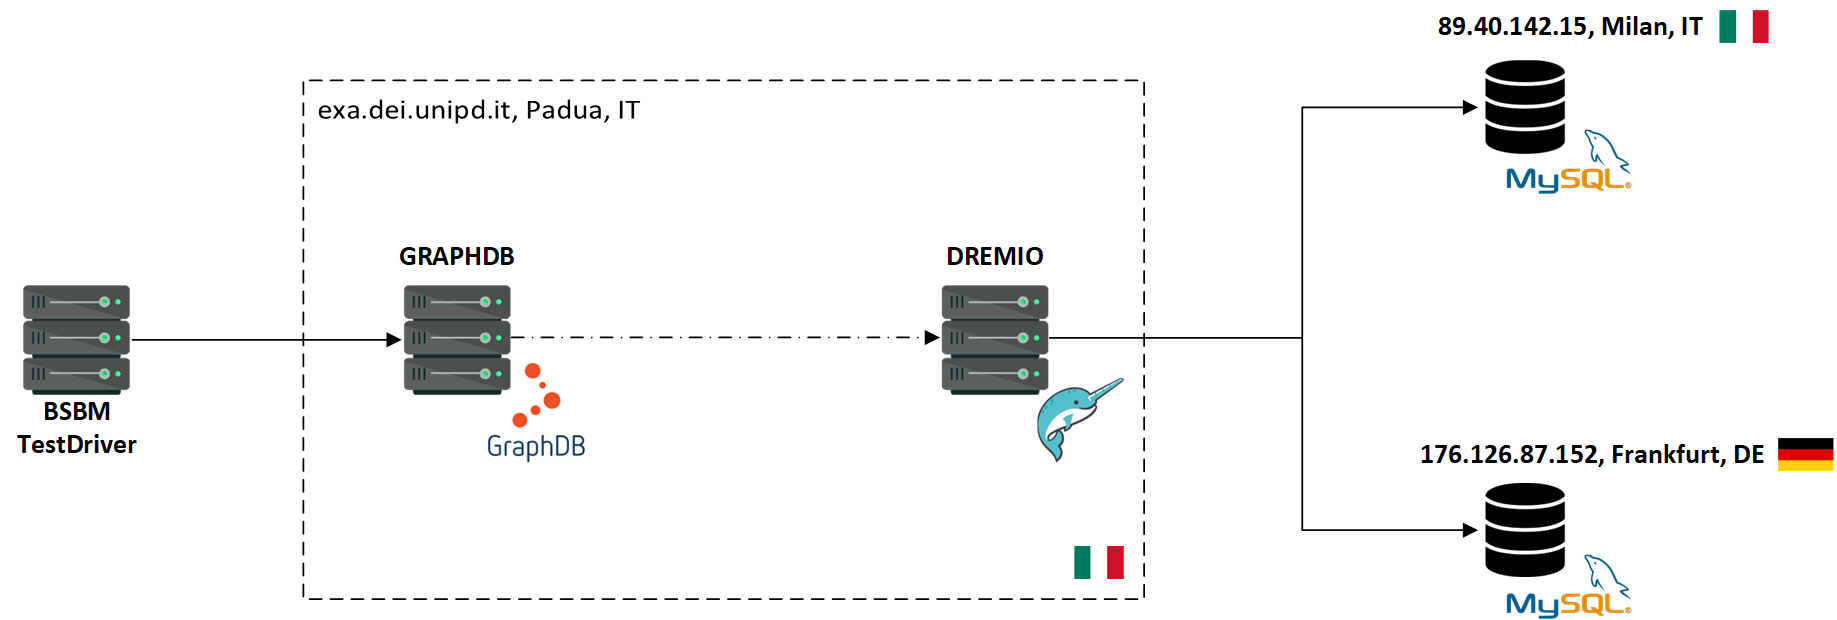
\includegraphics[width=16cm]{res/benchmark-setup.png}
    \caption{Architecture Setup for Benchmarking}
    \label{fig:benchmark-setup}
\end{figure}

\subsubsection{Benchmark Results}
We ran the TestDriver with the following parameters:
\begin{lstlisting}[language=bash, caption={BSBM TestDriver class execution}, label={lst:testdriver}]
    $ java -cp bin:lib/* benchmark.testdriver.TestDriver -runs 32 -w 4 -mt 4 -t 30000 http://localhost:7200/repositories/BSBM
\end{lstlisting}
For each query (12 in total), we ran them 32 times with 4 concurrent processes submitting queries. We excluded the first 4 queries from the measurements as a warm-up phase to eliminate any potential noise from caching mechanisms. Moreover, we set a timeout of 30 seconds for each query.

The first notable observation from results in Fig. \ref{fig:bsbmbenchmarkresults} is that the plots are complementary: this is expectable, as a one of the main causes for a low query rate can be for sure an high response time.
We can observe how Query 3 and Query 11 are performing poorly with respect to the others. As we will see in next section with other benchmarks, where we will compare resource consumption between Dremio and Ontop hosted in GraphDB, the component that usually is more resource-demanding and consuming is the virtualization system Dremio. This implies that an eventual bottleneck has to be caused at this level. By inspecting Queries 3 and 11, we can see how these two make use of extensive joins among tables that in our set up belongs to different sources as well as nested queries. This translates to a possible weakness of the proposed architecture while dealing with these case study, but that can surely be investigated and strengthen in future.
In general, our architecture was able, on average, to perform 15 queries per seconds from 4 concurrent processes acting as independent users. This represent a huge milestone, considering it is an embryonic study.
\\
\begin{figure}[!ht]
    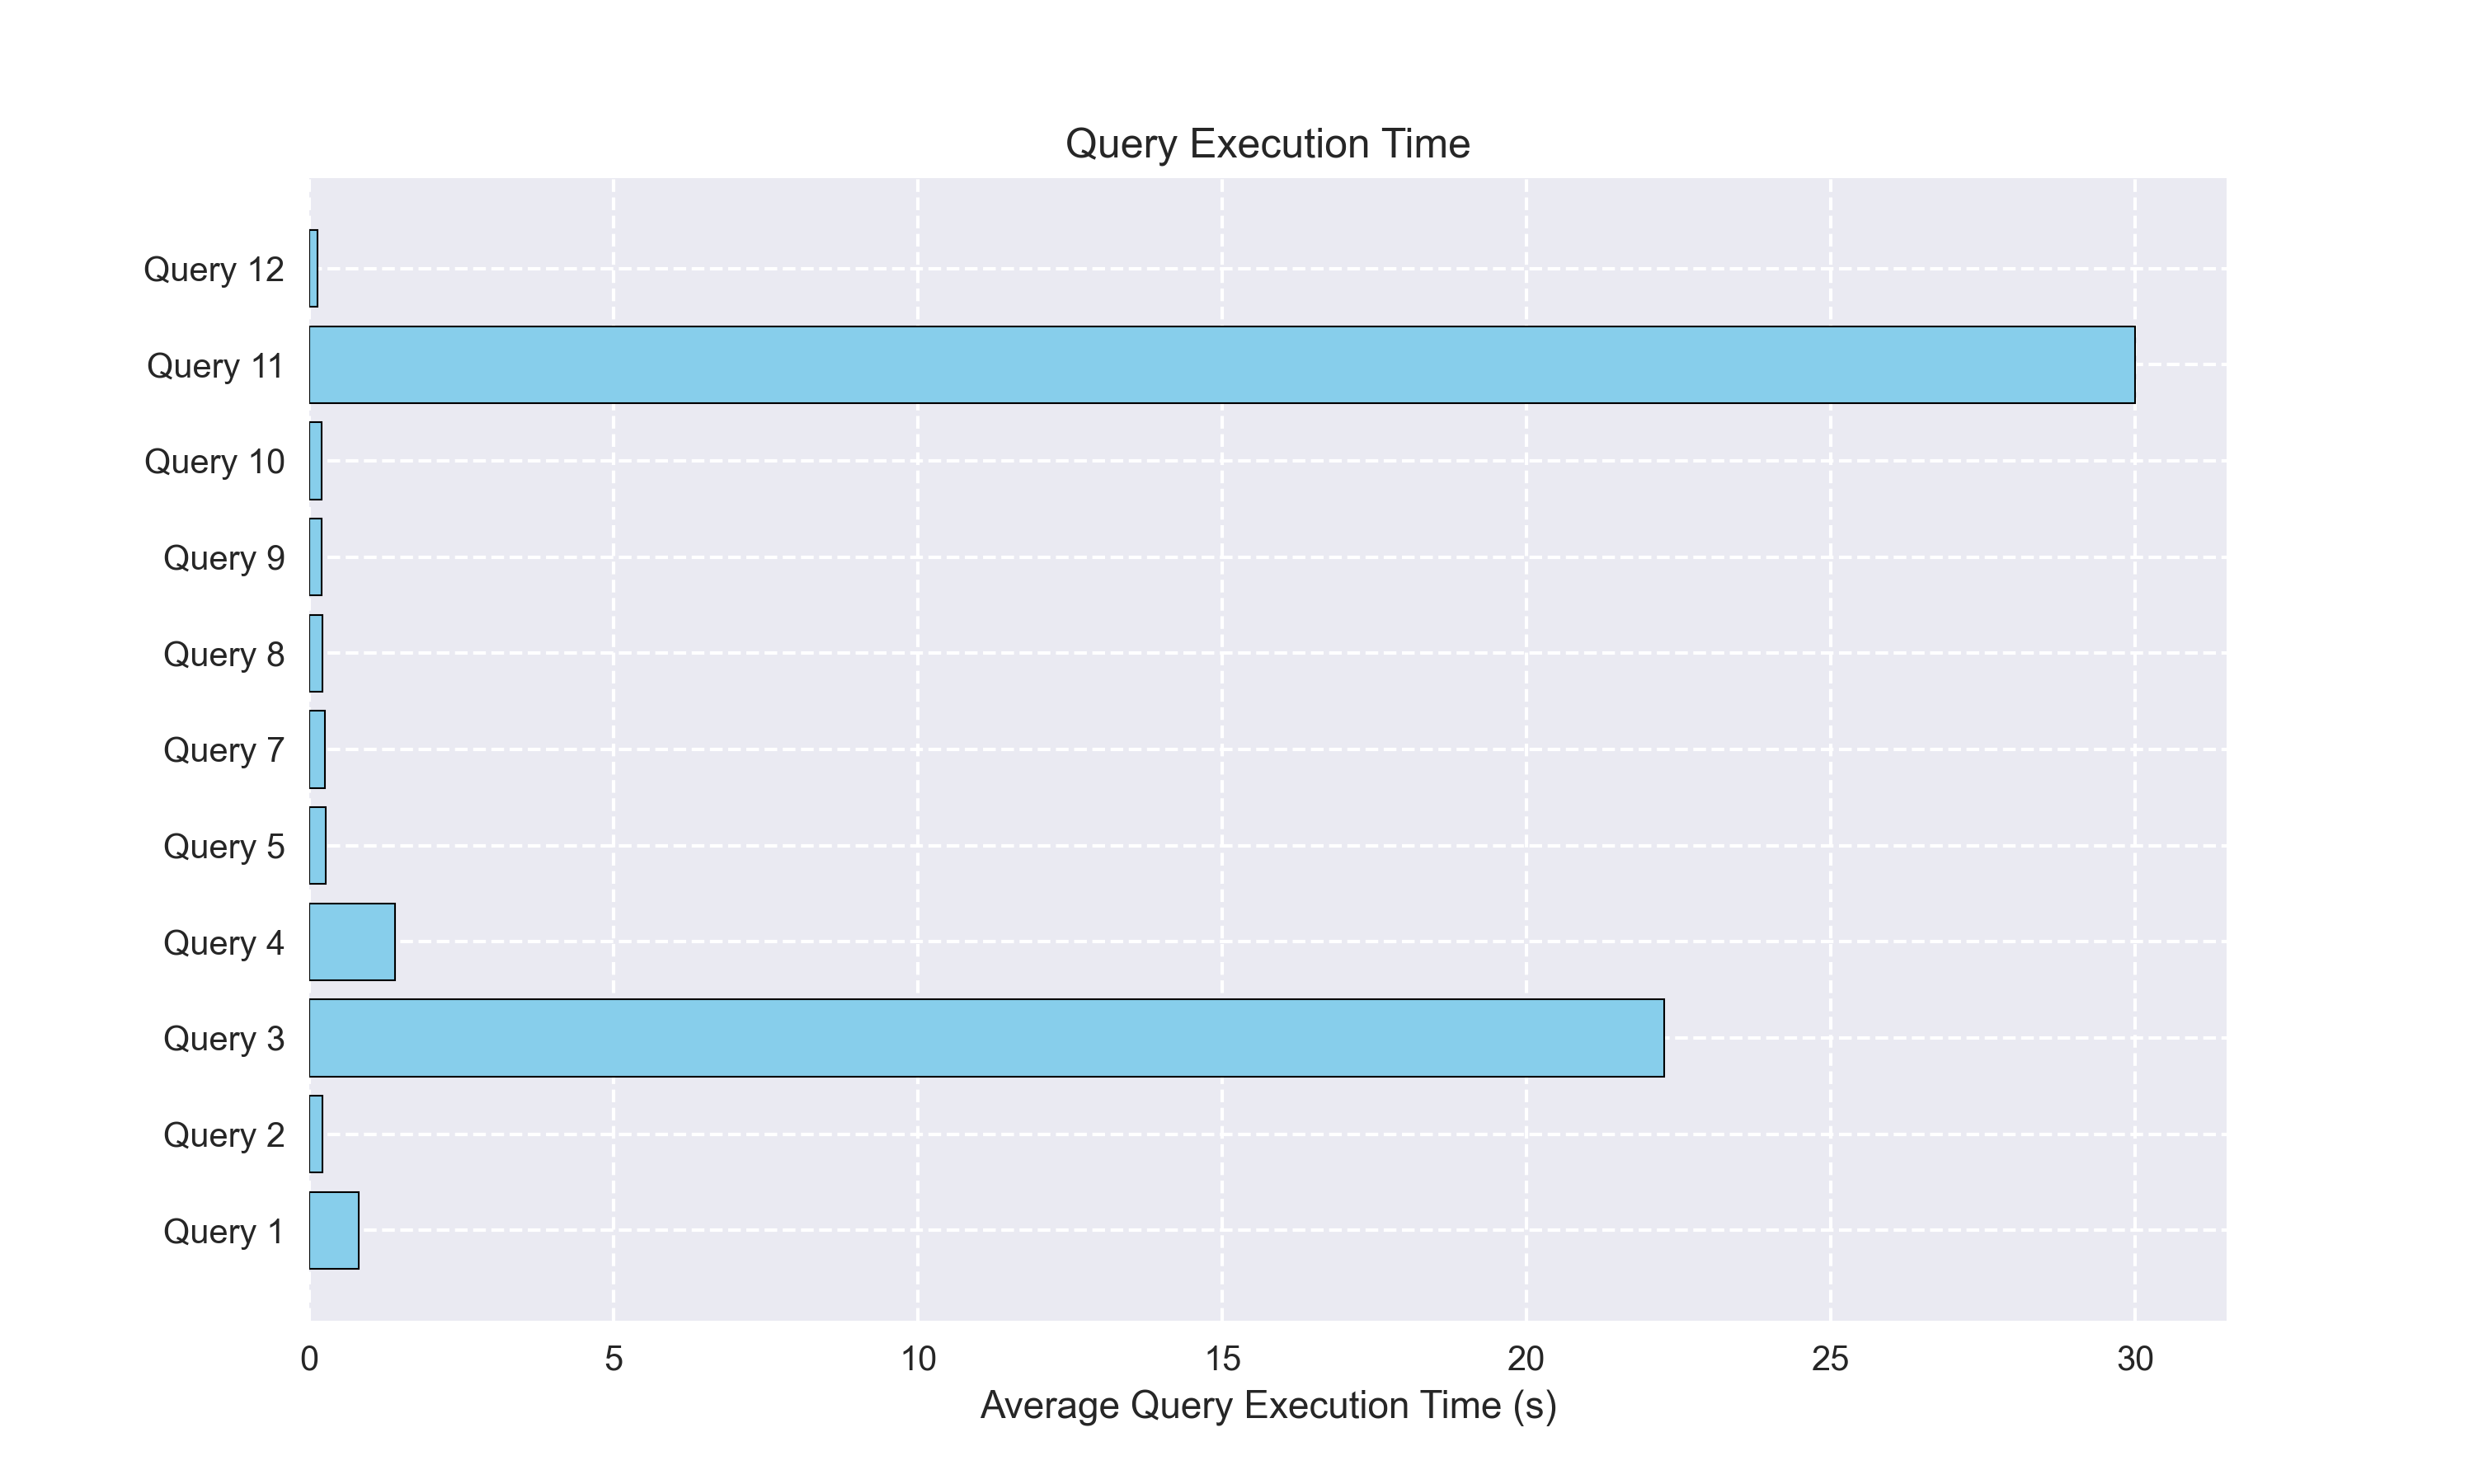
\includegraphics[width=16cm]{res/query_execution_time.png}
    \\
    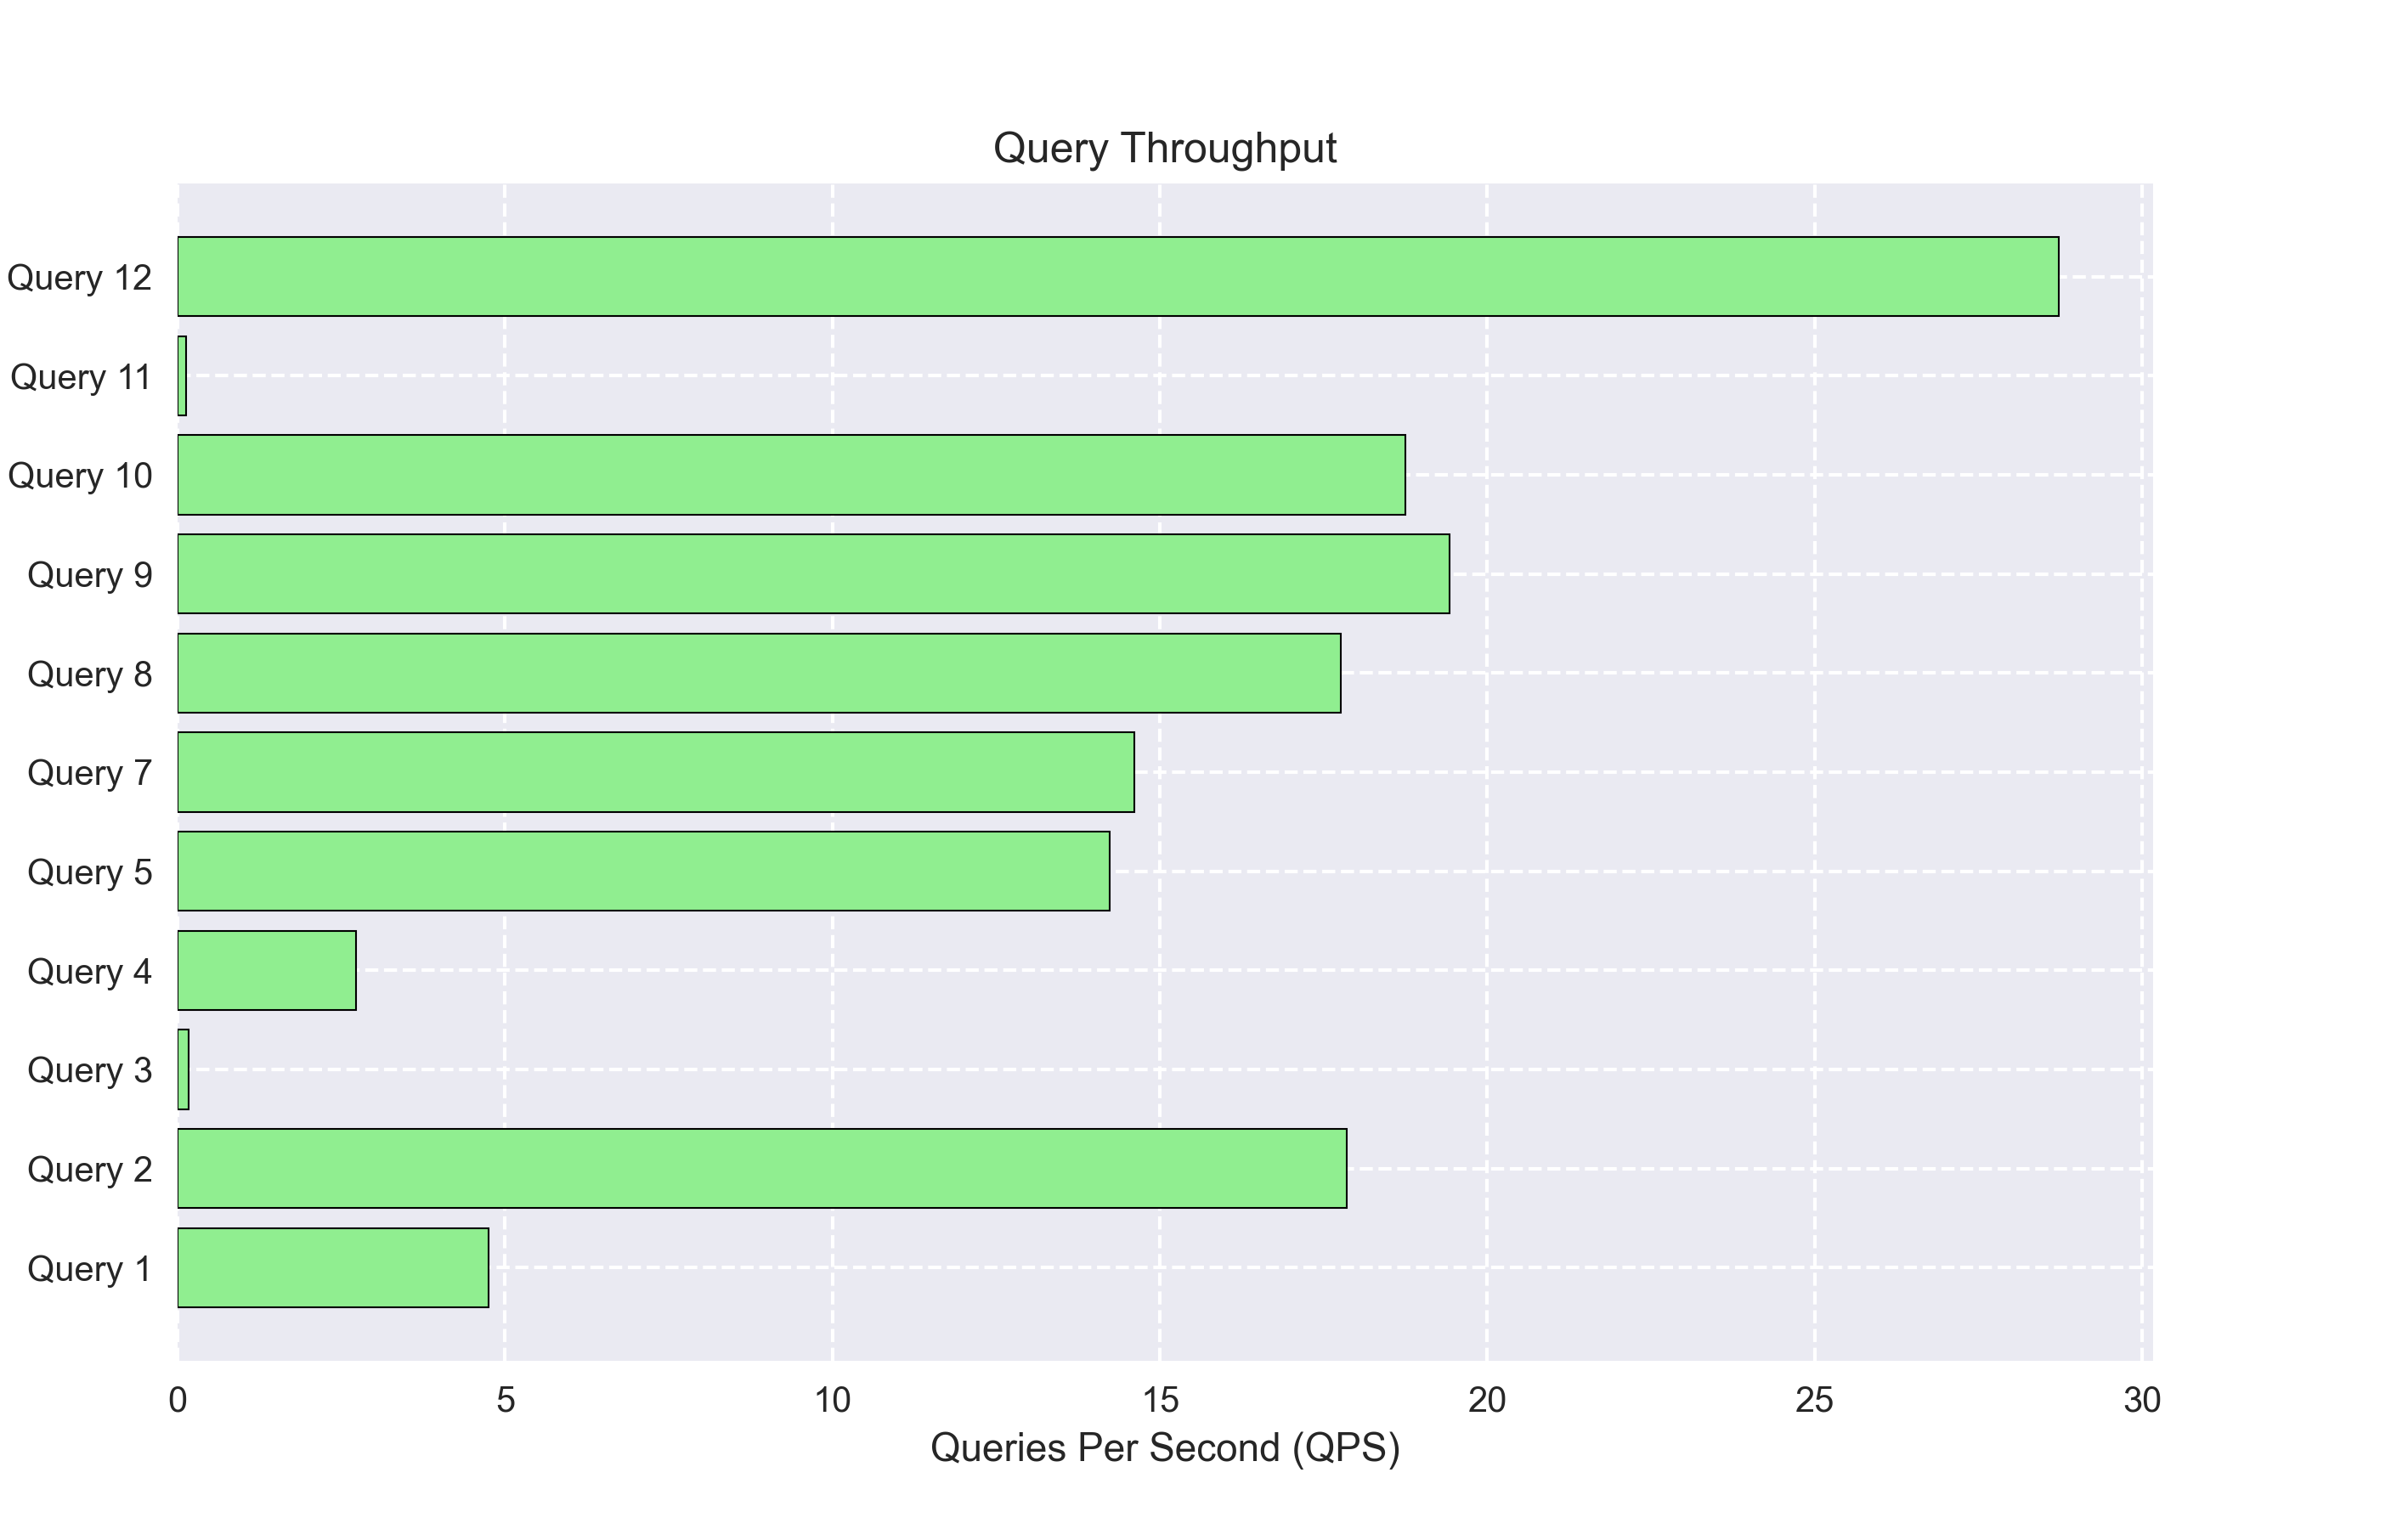
\includegraphics[width=16cm]{res/query_throughput.png}
    \caption{BSBM Benchmark Results}
    \label{fig:bsbmbenchmarkresults}
\end{figure}
\\

\section{Architecture Performance Benchmarking over Clinical Data}
In alignment with the methodologies presented in Section \ref{chp:dolci}, we conducted an extensive evaluation of our healthcare data architecture using our available clinical data. This benchmarking initiative was critical to validate the architecture's operational efficacy, specifically targeting its ability to handle real-world healthcare analytics tasks efficiently.
The benchmark framework was constructed around a custom-developed monitoring script. This script, integral to our testing methodology, was engineered to capture and log real-time \ac{CPU} and \ac{RAM} delta usage metrics by process ID.
\begin{lstlisting}[language=bash, caption={Custom Monitor Script for Performance Tracking}, label={lst}] 
#!/bin/bash

pid=$1
output_file=$2

# Get the number of CPUs
num_cpus=$(nproc)

# Time interval in seconds
interval=1

trap 'echo "Monitor stopped"; exit' SIGINT SIGTERM

if [ -z "$pid" ] || [ -z "$output_file" ]; then
    echo "Usage: $0 <PID> <output_file>"
    exit 1
fi

exec > $output_file

while true; do
    # Capture CPU times at the start of the interval
    start_utime=$(cat /proc/$pid/stat | cut -d " " -f 14)
    start_stime=$(cat /proc/$pid/stat | cut -d " " -f 15)
    start_total=$(cat /proc/stat | grep '^cpu ' | awk '{print $2+$3+$4+$5+$6+$7+$8}')

    # Capture the initial RAM usage
    start_ram=$(grep VmRSS /proc/$pid/status | awk '{print $2}')

    sleep $interval

    # Capture CPU times at the end of the interval
    end_utime=$(cat /proc/$pid/stat | cut -d " " -f 14)
    end_stime=$(cat /proc/$pid/stat | cut -d " " -f 15)
    end_total=$(cat /proc/stat | grep '^cpu ' | awk '{print $2+$3+$4+$5+$6+$7+$8}')

    # Capture the end RAM usage
    end_ram=$(grep VmRSS /proc/$pid/status | awk '{print $2}')

    # Calculate the deltas for CPU
    delta_process=$(( (end_utime + end_stime) - (start_utime + start_stime) ))
    delta_total=$(( end_total - start_total ))

    # Calculate CPU usage as a percentage
    cpu_usage=$(awk "BEGIN {printf \"%.2f\", (${delta_process} / ${delta_total}) * 100 * ${num_cpus}}")

    # Calculate RAM usage change if needed
    ram_usage_change=$(( end_ram - start_ram ))

    echo "$(date +'%Y-%m-%d %H:%M:%S') CPU Usage: ${cpu_usage}% | RAM Usage Change: ${ram_usage_change} kB"

done
\end{lstlisting}

The benchmarking trials were designed to assess the architecture's performance by running the same analytical query we considered for the use case analysis in Chapter \ref{chp:usecase} that simulate typical data processing tasks encountered in clinical settings. During these tests, our monitoring script provided continuous feedback on system performance, enabling a comprehensive analysis of \ac{CPU} and \ac{RAM} usage across different operational states.
Illustrated in Figures \ref{fig:bench_Dremio} and \ref{fig:bench_GraphDB}, the system's response to the execution of computationally intensive queries reveals significant insights into its dynamic resource allocation and management capabilities.
\begin{figure}[!ht] 
    \centering 
    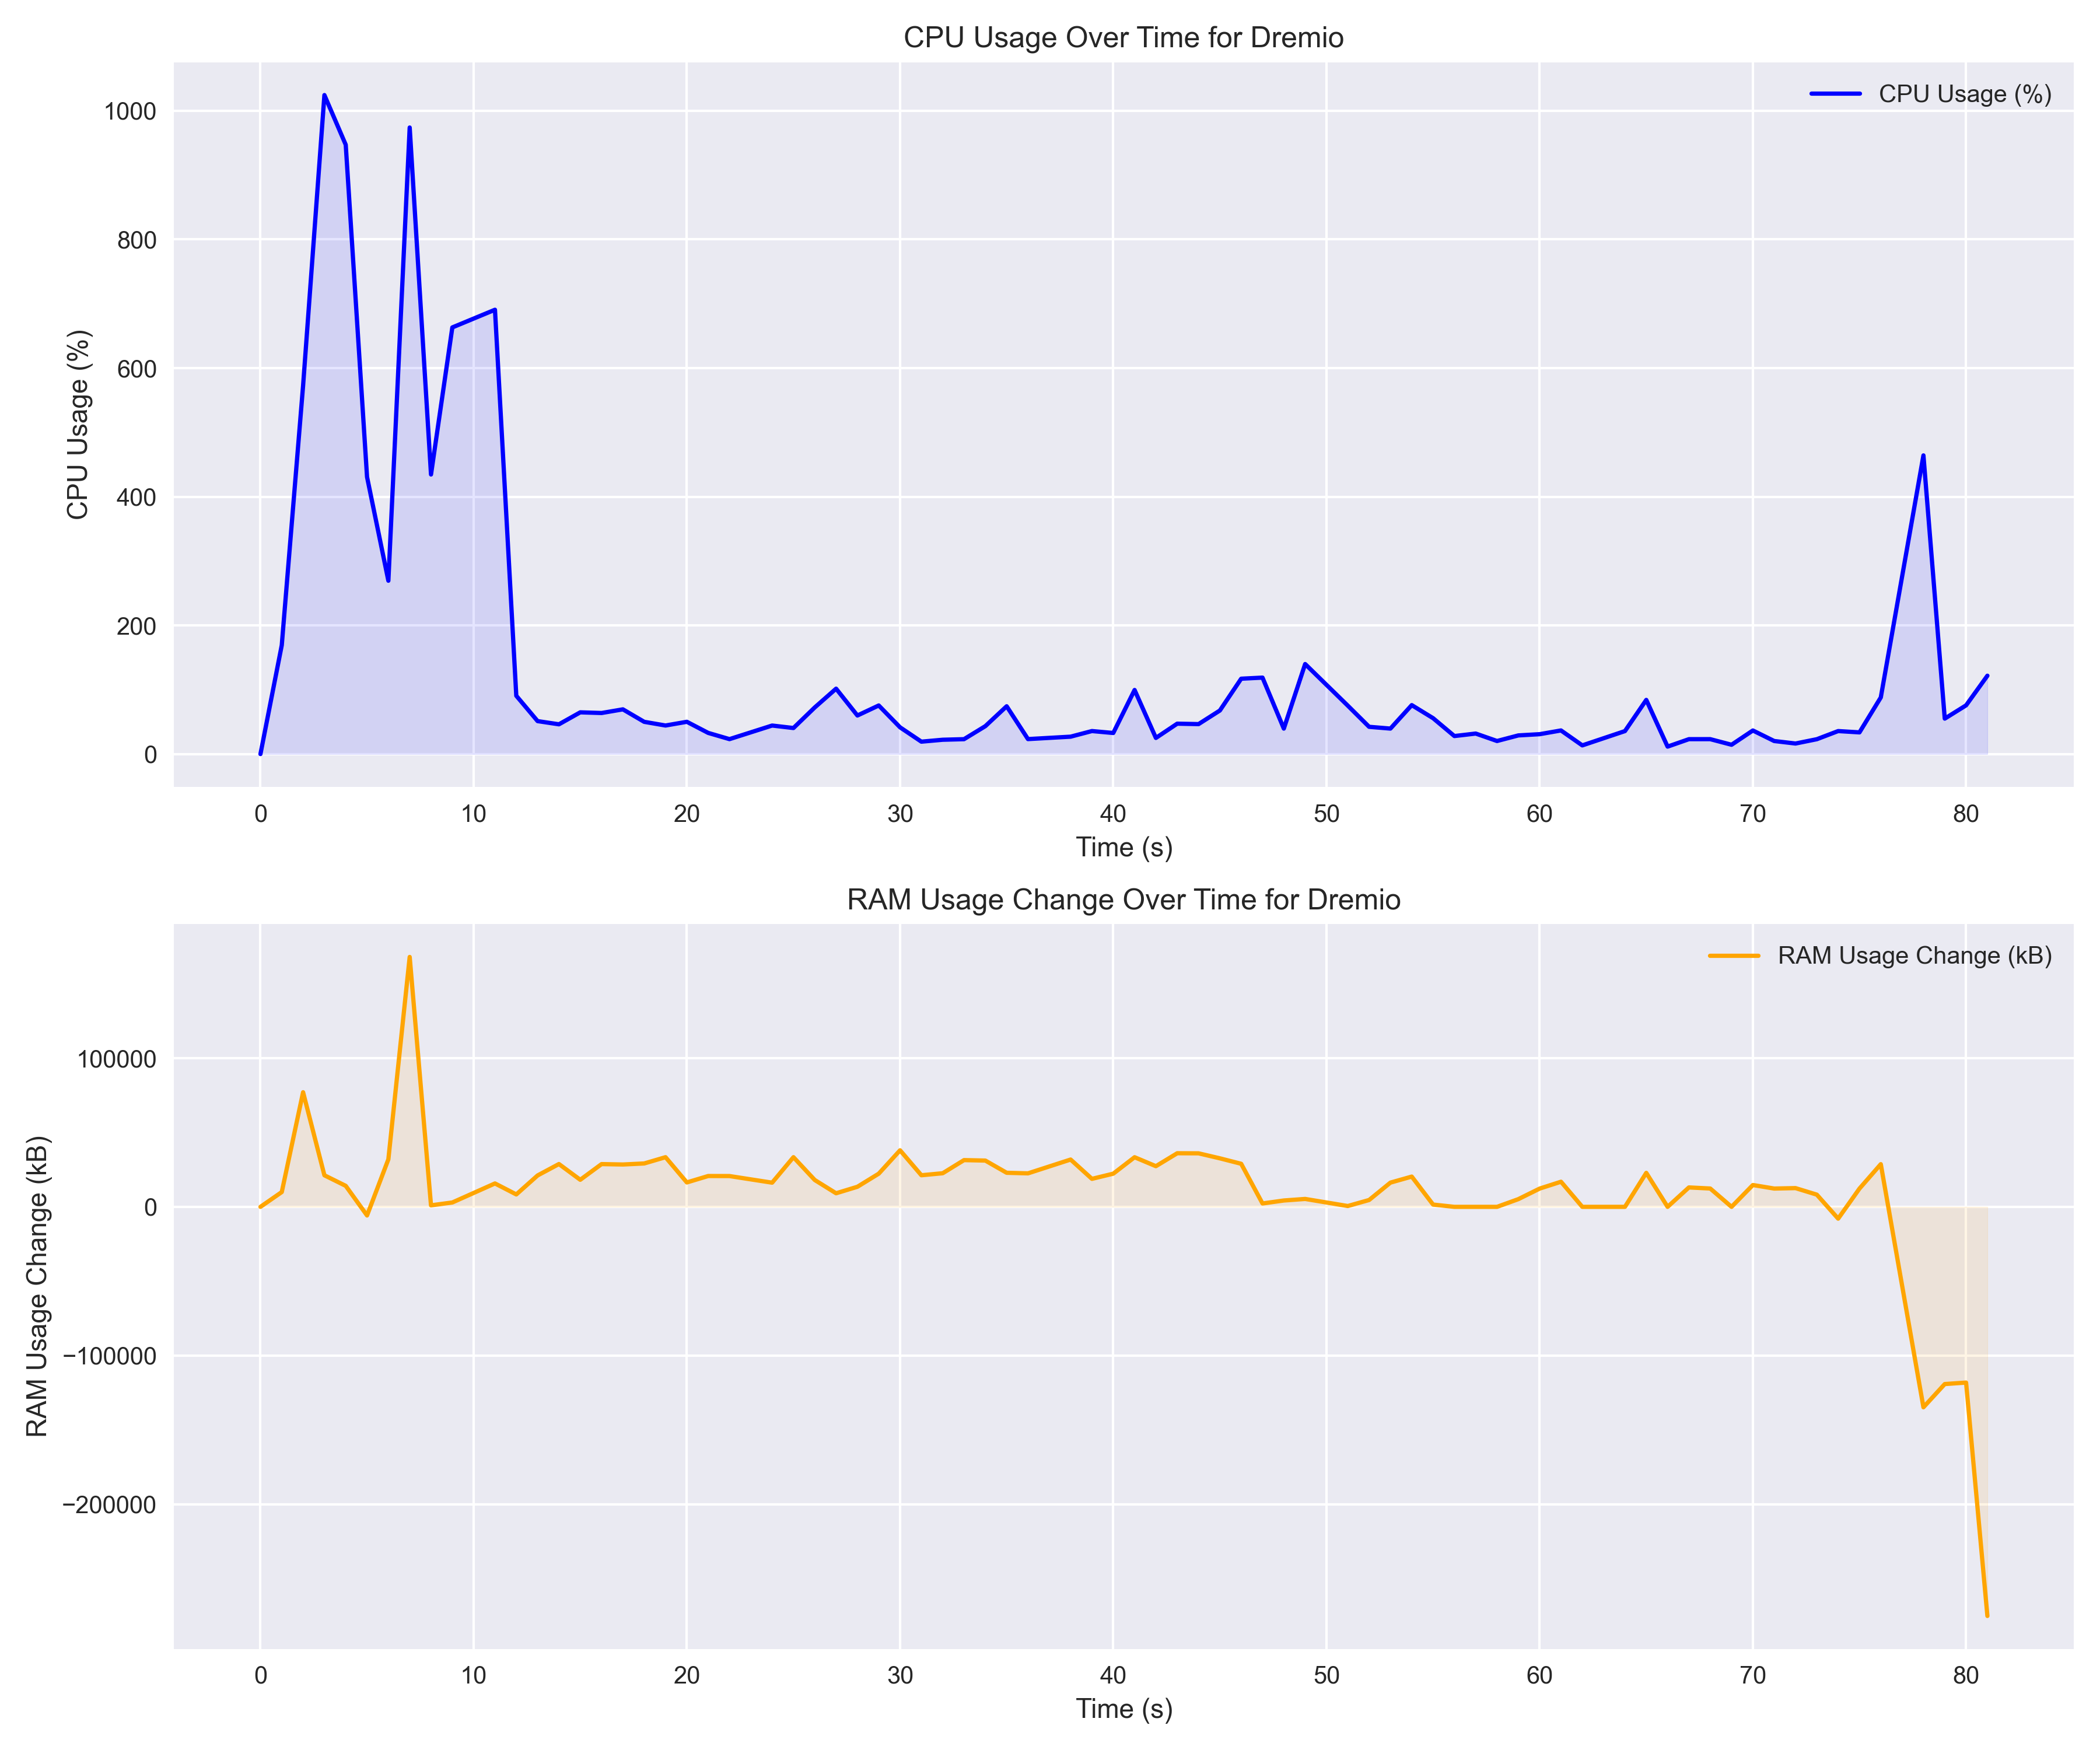
\includegraphics[width=11.6cm]{res/Dremio_usage_plot.png} 
    \caption{\ac{CPU} and \ac{RAM} usage over time for Dremio during benchmarking} 
    \label{fig:bench_Dremio}
\end{figure}
\begin{figure}[!ht] 
    \centering 
    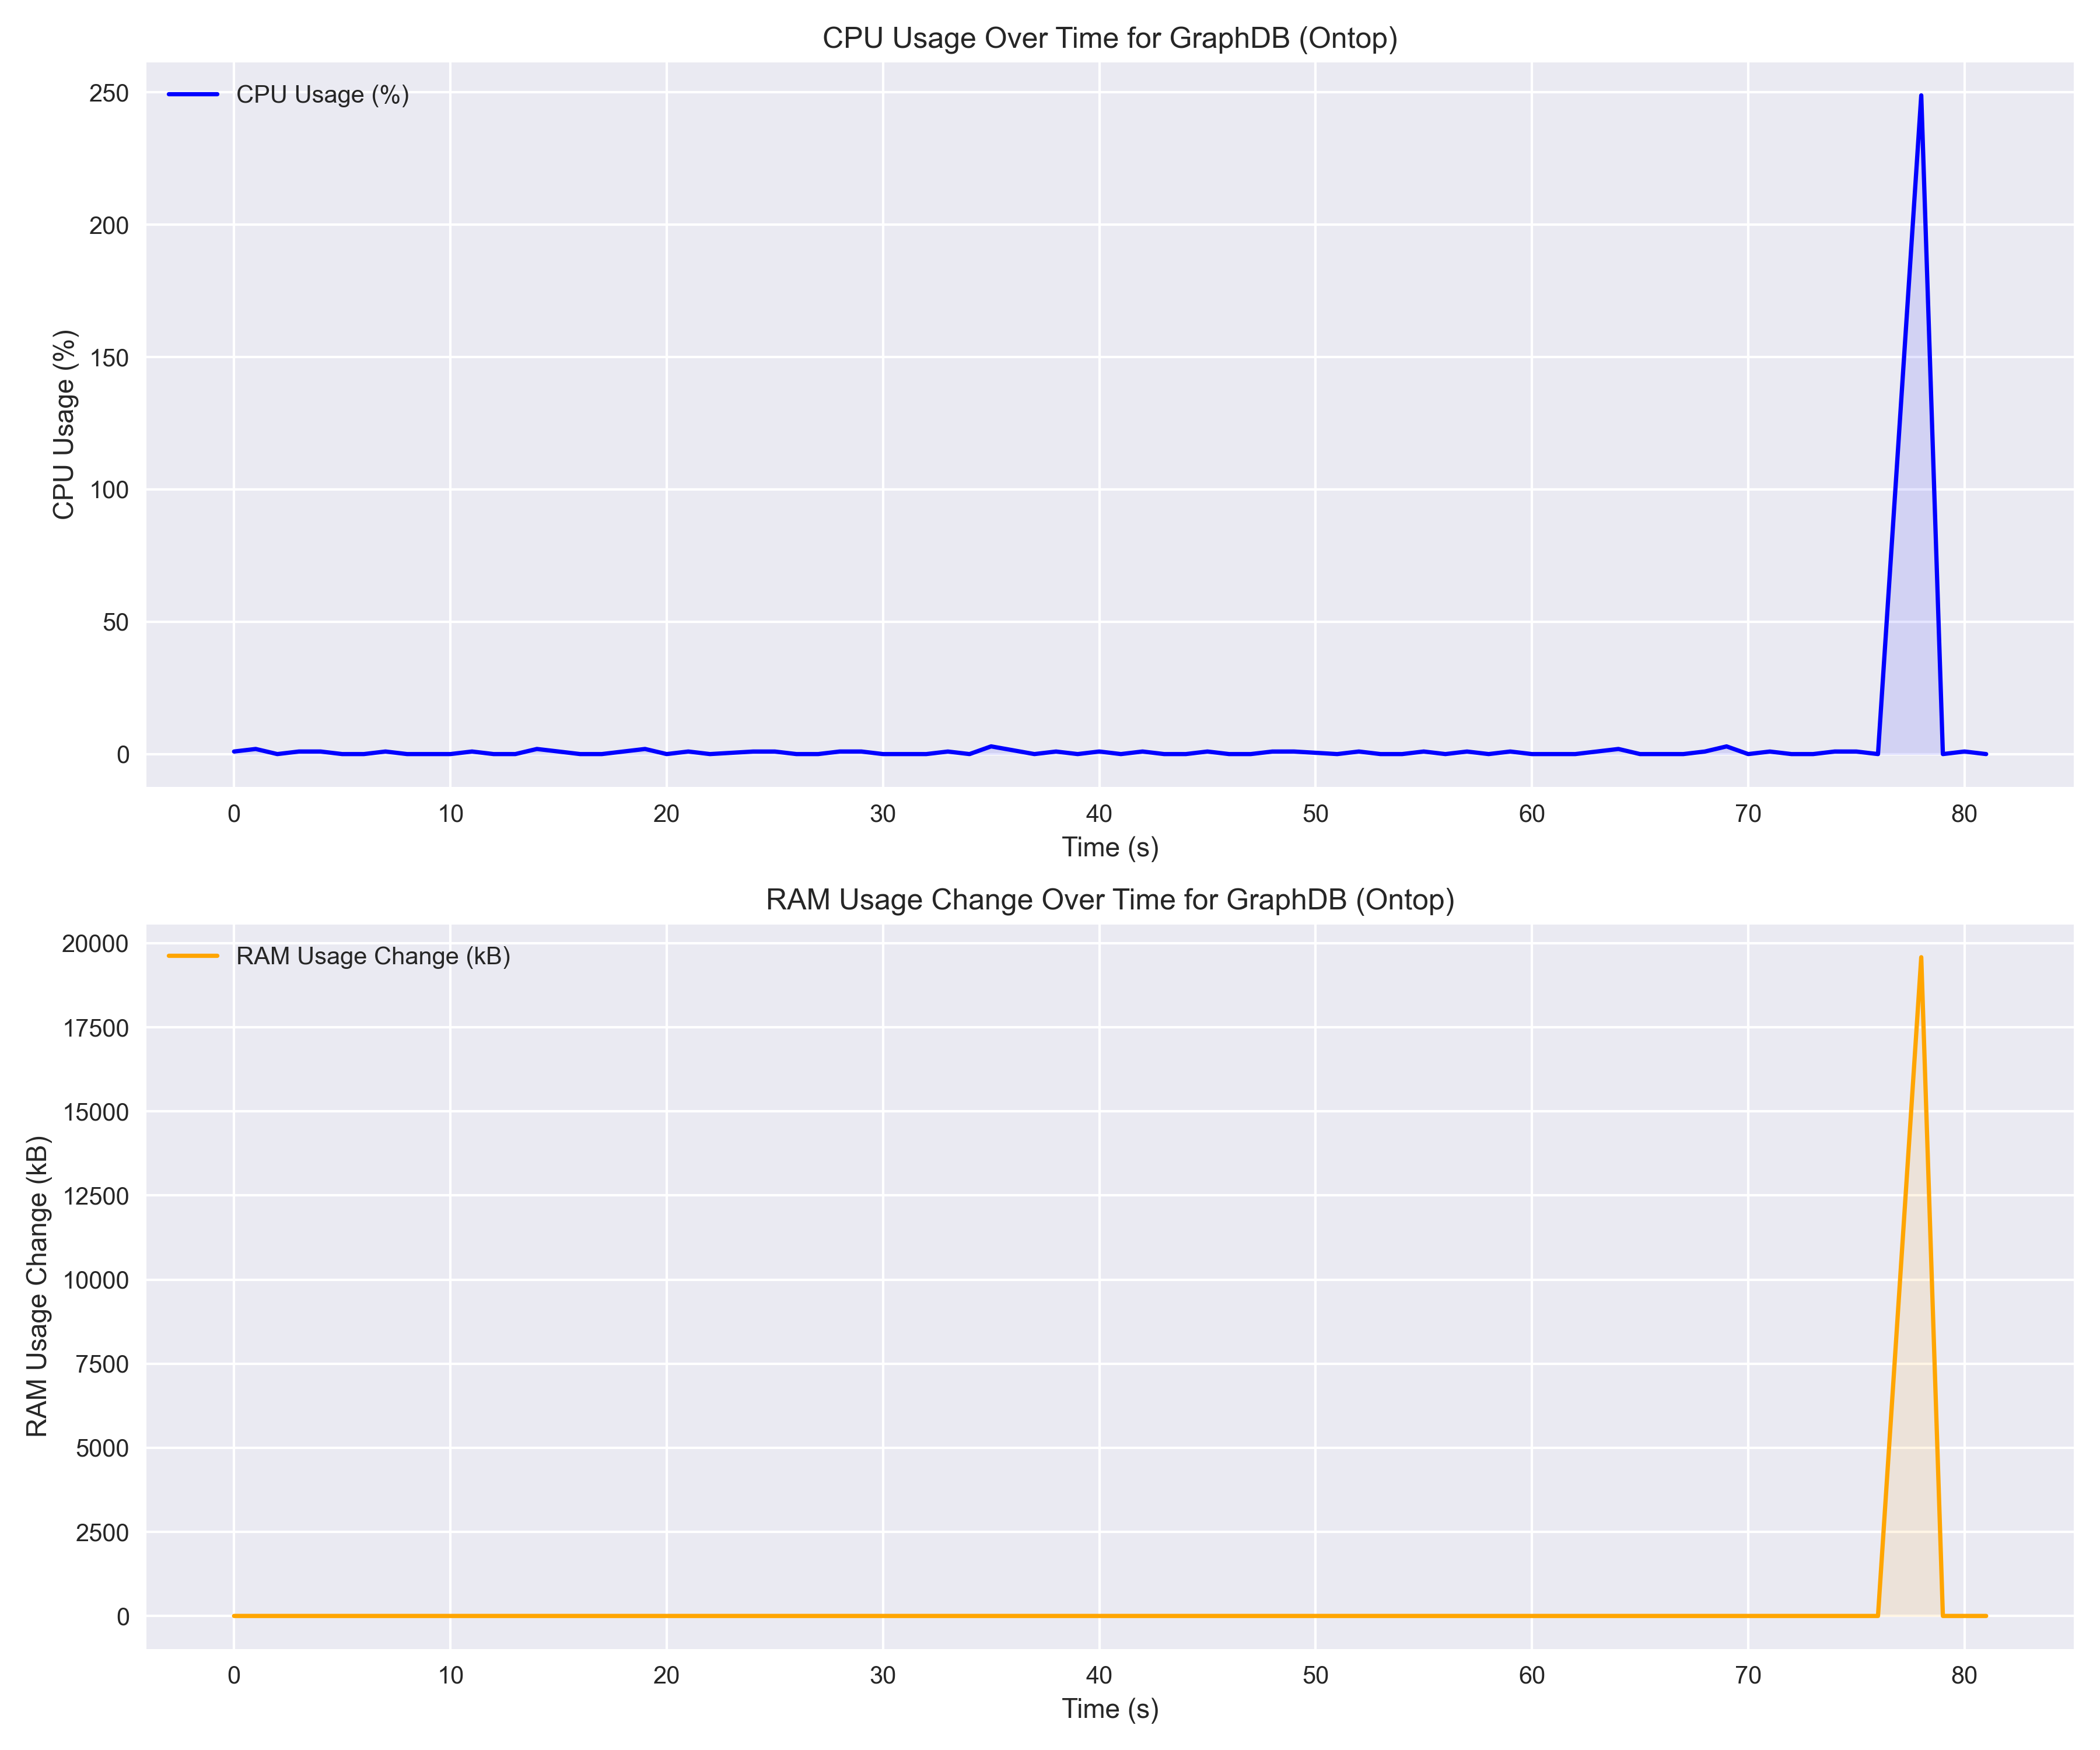
\includegraphics[width=11.6cm]{res/GraphDB (Ontop)_usage_plot.png} 
    \caption{\ac{CPU} and \ac{RAM} usage over time for GraphDB (Ontop) during benchmarking} 
    \label{fig:bench_GraphDB}
\end{figure}
We analyzed the output from the two monitoring daemons, synchronizing samples at the moment the query was submitted by inspecting the query logs in Dremio. This allowed us to generate superimposable plots for independent analysis of \ac{CPU} load and variations in \ac{RAM} usage.
Notably, the trends for both \ac{CPU} and \ac{RAM} usage appear almost flat in GraphDB, except for a spike nearly coinciding with the completion of query execution. In contrast, Dremio exhibits non-negligible resource consumption throughout the entire duration of the query execution, with spikes occurring both at the beginning and the end of the process.
These phenomena may be explained by the fact that, upon submission, query execution in GraphDB does not initially involve resource-intensive activities, whereas in Dremio, it is necessary to exploit the views structure of the submitted query to begin fetching data from various sources. The spikes at the end are likely related to the combination of results from these sources and the activities involved in presenting the data to the user.
The occurrence of these spikes suggests potential areas for optimization, which could be crucial for improving the system's efficiency and responsiveness, especially under peak load conditions.
In conclusion, this benchmarking exercise has not only validated the robustness of our healthcare data architecture but also identified specific enhancement opportunities that can significantly improve system performance.


\section{Summary and Conclusions}
This chapter provided a detailed overview of the benchmarking process for our federated data architecture, particularly focusing on its performance and operational efficiency in the realm of genomics research. Through a series of meticulously designed benchmarks, we evaluated the architecture's ability to handle complex data interactions and manage computational resources effectively, ensuring its suitability for deployment in high-demand genomics research environments.
The benchmarks detailed in this chapter utilized state-of-the-art methodologies, including the Berlin \ac{SPARQL} Benchmark and the \ac{SEASHELL} framework for healthcare data lakes, to provide a comprehensive assessment of the architecture's performance across various scenarios. These tests revealed both the strengths and potential areas for improvement in our system, highlighting the critical need for continual optimization.